\section{Results}
\label{sec:results}

Every number in this section is generated from \file{results/*.json} by \file{analysis/numbers.py}, which is locked, or by \file{tools/paper_numbers.py}, which computes descriptive counts only.

\subsection{Sample}
\label{sec:sample}

The \StudyK{} study benchmarks hold \AnalysisRowsTotal{} analysis rows.
Five reasons remove a row from the primary sample, applied in a fixed order so that each row is counted once.
Own-lineage rows, whose primary parent was the same solver, number \ExclOwnLineage{}; they are the sample for H2.
Multi-source rows number \ExclMultiParent{}, and rows that are novel or have no parent number \ExclNovel{}.
Cross-solver rows in which the child's or the parent's family is Unknown or Multi number \ExclUnknownFamily{}.
Rows before the confirmatory window number \ExclOutsideWindow{}.
That leaves \PrimaryRowsTotal{} primary rows.
Solvers whose primary rows all share one outcome carry no information in the conditional model, and the fits use the remaining \FitRowsTotal{} rows.

Among analysis rows, the primary parent came from declared attribution for \DeclaredShare{}, from a base named in the note for \TextShare{}, and from tree distance for \TreeShare{}.
Novel rows are \NovelShare{}, rows with no candidate parent \NoParentShare{}, and multi-source rows \MultiShare{}.
Across all analysis rows with a single parent and two known families, the four treatment cells hold \CellOwnSame{} own-lineage same-family rows, \CellOwnSwitch{} own-lineage switches, \CellOtherSame{} cross-solver same-family rows and \CellOtherSwitch{} cross-solver cross-family rows.
Building on another vendor's work is therefore the common case on these leaderboards, not the exception.
Figure~\ref{fig:flow} breaks the cross-solver rows down by parent and child family.
Anthropic and OpenAI models dominate both sides, and the largest cross-family flows run between them.

\begin{figure}[t]
\centering
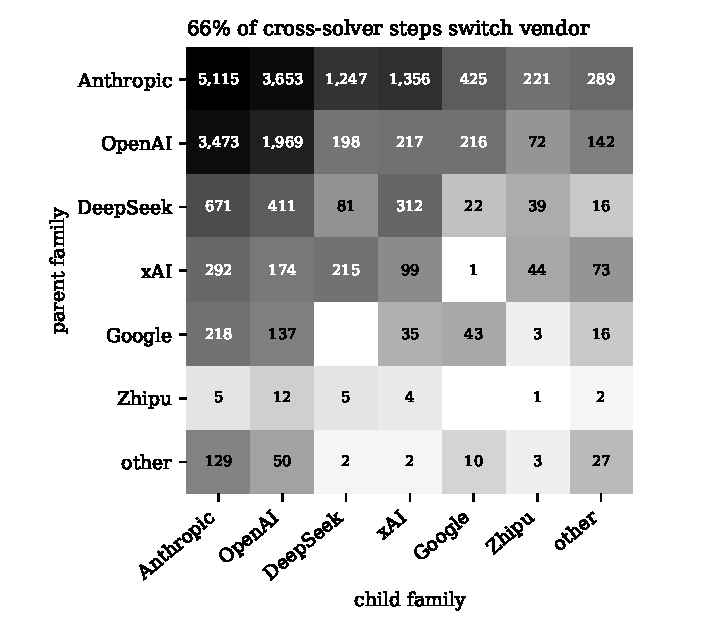
\includegraphics[width=0.62\linewidth]{figures/paper_family_flow.pdf}
\caption{Cross-solver single-parent rows with two known families, by parent family (rows) and child family (columns), pooled over the \StudyK{} study benchmarks. The six largest families are shown; ``other'' folds the rest, so its diagonal cell mixes families. Off-diagonal cells are cross-family steps. Source: treatment frames from \file{analysis/dataset.py}; figure by \file{tools/paper_figures.py}.}
\label{fig:flow}
\end{figure}

\subsection{Primary estimate}
\label{sec:primary}

Pooled across all \PooledK{} benchmarks, the odds ratio of promotion for cross-family against same-family rows is \PooledOR{}, with a 95\% interval of \PooledORLow{} to \PooledORHigh{} and a 90\% interval of \PooledORNinetyLow{} to \PooledORNinetyHigh{}.
The 90\% interval lies inside the margin of \MarginLow{} to \MarginHigh{}, and the 95\% interval includes 1.
The pre-registered verdict is \emph{\PooledVerdict{}}.
No benchmark was excluded for lack of a finite estimate.
Figure~\ref{fig:forest} shows the per-benchmark estimates and the pooled interval.

The verdict depends on the widened margin.
Under the original margin of $[0.80, 1.25]$, the upper end of the 90\% interval, \PooledORNinetyHighFine{}, lies above 1.25, and the verdict would be inconclusive.
The margin was widened by the rule fixed in the specification before any analysis: the power gate, run on treatment counts and simulated outcomes only, gave \PowerEquivalence{} at the original margin and \PowerWidened{} at the widened one (Section~\ref{sec:equivalence}).
The widened margin and its reason are part of the text locked by \texttt{prereg-v1}, and the confirmatory run happened after the tag.

The between-benchmark variance is $\tau^2 = \PooledTauSquared{}$, with a Q-profile interval of \PooledTauSquaredLow{} to \PooledTauSquaredHigh{}.
The equivalence verdict is a statement about the average effect across benchmarks.
A 90\% prediction interval for the effect on a new benchmark, computed from $\tau^2$ and the pooled standard error of \PooledSE{} with a $t$ distribution on $k-2$ degrees of freedom, runs from \PredLow{} to \PredHigh{} and extends past the margin at both ends.
This interval was not pre-registered.
The data are consistent with no effect on average while leaving room for modest effects, in either direction, on individual benchmarks.

Every benchmark's fit used Firth's penalised likelihood rather than the conditional fit.
In each benchmark the conditional fit showed separation or failed its convergence checks, which is the condition the pre-registration names for the fallback (Section~\ref{sec:model}). In the frames examined, the separation came from sparse family indicators and spline terms, not from the treatment.
With Firth, solver indicators enter as fixed effects instead of being conditioned out.

\begin{figure}[t]
\centering
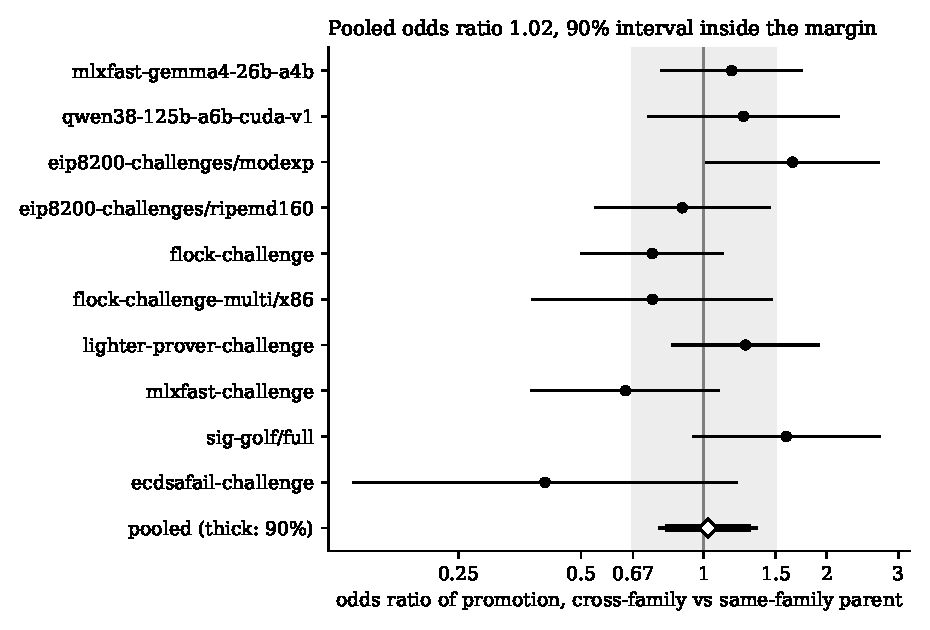
\includegraphics[width=0.92\linewidth]{figures/paper_forest_primary.pdf}
\caption{Odds ratio of promotion for cross-family against same-family cross-solver rows, by benchmark with 95\% intervals, and the pooled estimate with its 95\% (thin) and 90\% (thick) intervals. The shaded band is the margin $[0.67, 1.50]$. Source: \file{results/confirmatory.json}; figure by \file{tools/paper_figures.py}.}
\label{fig:forest}
\end{figure}

\subsection{ECDSA.Fail}
\label{sec:ecdsa}

On ECDSA.Fail alone the odds ratio is \BenchJOR{}, with a 95\% interval of \BenchJORLow{} to \BenchJORHigh{} and a 90\% interval of \EcdsaNinetyLow{} to \EcdsaNinetyHigh{}, from \BenchJFitRows{} primary rows and \BenchJStrataKept{} informative solvers.
The verdict is \emph{\CaseStudyVerdict{}}.
The point estimate runs against pollination, but the interval is compatible with anything from a strong negative effect to a small positive one.
Section~\ref{sec:equivalence} showed before the lock that a single-benchmark verdict there would almost surely be inconclusive.
As a member of the secondary family, ECDSA.Fail's H1 test has $p = \SecHOneJP{}$ and a Holm-adjusted $p = \SecHOneJPHolm{}$.

\subsection{Secondary tests}
\label{sec:secondary-results}

Table~\ref{tab:secondary} in Appendix~\ref{app:secondary} lists every secondary test.
\HolmFamilySize{} tests passed the minimum-events gate and form the Holm family: ECDSA.Fail's H1, H4 on each of the \StudyK{} benchmarks, and H5.
No member is significant after correction; the smallest Holm-adjusted $p$ is \HolmMinP{}.
All H2 tests fell below the gate, because own-lineage family switches are rare and few of them were promoted, so H2 is descriptive on every benchmark.
H3a and H3b were also below the gate everywhere.
Large jumps among cross-solver promotions number between 1 and 10 per benchmark in the smaller arm, and plateau breaks at most one.
The per-benchmark estimates in Figure~\ref{fig:forest} are components of the pooled estimate, not separate tests.
One of them, \ExcludesOneBench{}, has a 95\% interval that excludes 1 (unadjusted $p = \ExcludesOneP{}$); among ten benchmarks, about half of one such interval is expected by chance.

\subsection{Exploratory analyses}
\label{sec:exploratory}

These analyses are exploratory and uncorrected.
E1 compares \EOneMultiRows{} multi-family or multi-source rows with \EOneSingleRows{} single-family, single-parent rows.
Most benchmarks have too few multi rows for a stable estimate, and the per-benchmark results are in \file{results/exploratory.json}.
E2 splits each benchmark's analysis rows into thirds by time and pools H1 within each third.
The pooled odds ratios are \ExploreEThirdOneOR{}, \ExploreEThirdTwoOR{} and \ExploreEThirdThreeOR{} for the first, second and last third.
